\documentclass{article}
\usepackage[T2A]{fontenc}
\usepackage[utf8]{inputenc} 
\usepackage[russian]{babel} %  пакет для поддержки русского языка
\usepackage{amsmath} % математические символы и формулы 
\usepackage{graphicx}
\usepackage{amssymb}
\usepackage{listings}
\usepackage{xcolor}
\usepackage{hyperref}
\usepackage{needspace}
\usepackage{caption}
\usepackage{listingsutf8}
\lstset{inputencoding=utf8, extendedchars=\true, keepspaces=true, basicstyle=\rmfamily}
\usepackage{float} % позволяет контролировать плавающие объекты, такие как изображения и таблицы.


\begin{document}
\begin{titlepage}
\centering
\textbf{\LARGE АНО ПО "ИТ ХАБ"}

 
\vspace{1cm}

\textbf{\LARGE Отчёт по 1 КТ}

\vspace{1cm}
    
%\title{\textbf{\LARGE КТ: Линейные алгоритмы}}
%\maketitle
\textbf{\LARGE Локальная разработка. Линейные алгоритмы}

\vfill

\begin{flushright}
\textbf{\normalsize Выполнил: Бараш Илья} \\
\textbf{\normalsize Группа: 3ИБ1}
\end{flushright}
    
\vspace{1cm}
\centering
\textbf{\Large Москва, 2024}
\end{titlepage}

\newpage


\section{Постановка задачи}

На шахматной доске расположены Белый король, черная ладья и слон. Нужно определить, есть ли угроза королю, и если да, то от кого? Слон ходит по диагоналям, ладья по горизонталям и вертикалям.

\section{Вербальная модель решения}

Необходимо получить координаты белого короля, чёрных слона и ладьи для проверки, находится ли король под угрозой от слона или ладьи. Для определения угрозы королю от ладьи или слона также проверяется наличие другой фигуры, которая может блокировать угрозу между фигурой и королем.

\section{Математическая модель решения}

\resizebox{\textwidth}{!}{%
    \parbox{\textwidth}{%
    \begin{align*}
    &\text{Пусть } (x_1, y_1) \text{ -- координаты короля, } (x_2, y_2) \text{ -- координаты слона, } (x_3, y_3) \text{ -- координаты ладьи.} \\
    &\text{Угроза королю существует, если:} \\
    &\text{1. Король находится на одной горизонтали или вертикали с ладьей: } (x_1 = x_2) \lor (y_1 = y_2) \\
    &\text{2. Расстояние между королем и слоном по диагонали равно 1: } (|x_1 - x_3| = |y_1 - y_3|) \lor (|x_1 - x_3| = |y_3 - y_1|)
    \end{align*}
    }
}
\newpage
\section{Блок-схема}

\begin{center}
\needspace{6\baselineskip}
    \centering
    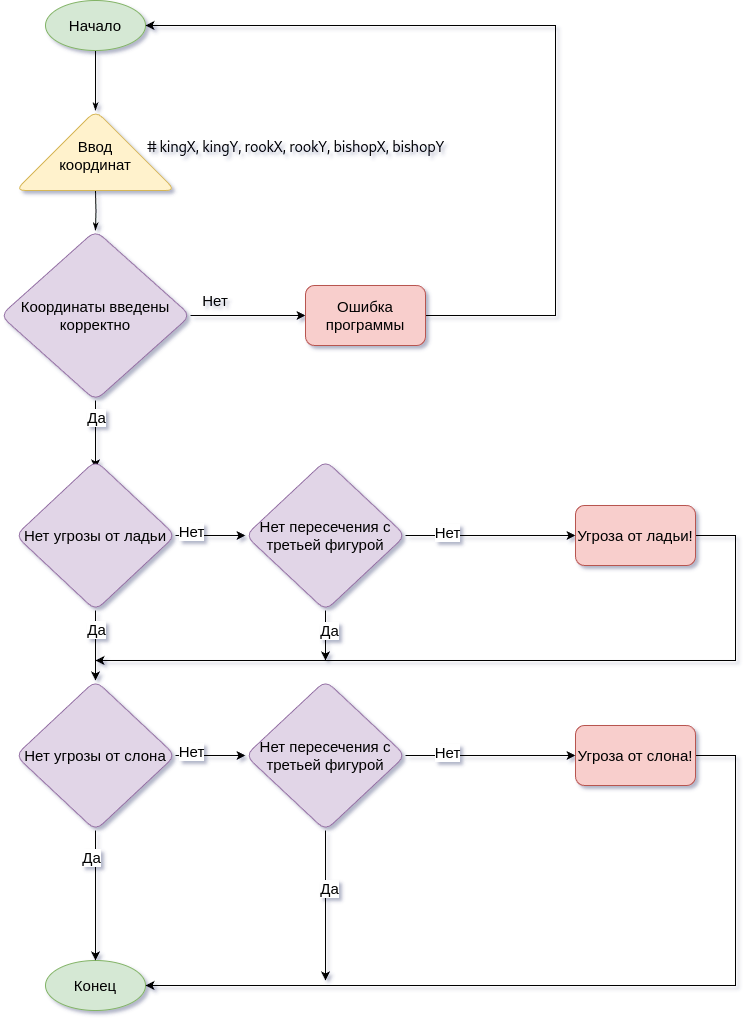
\includegraphics[width=0.9\textwidth]{chess_block_schema.drawio.png}
    \captionof{figure}{Блок-схема}
    \label{fig:chess block schema}

\end{center}

\newpage
\section{Программа на языке высокого уровня}

\begin{center}
%\begin{figure}[H]
\needspace{6\baselineskip}
\begin{lstlisting}[language=C++, caption=Решение на C++ (часть 1), numbers=left,frame=single, keywordstyle=\color{blue},commentstyle=\color{green}, stringstyle=\color{red}, showstringspaces=false, breaklines=true, linewidth=\linewidth,]
int main() {
    int kingX, kingY, rookX, rookY, bishopX, bishopY;

    // Ввод позиций фигур
    cout << "Введите позицию белого короля (x y): ";
    cin >> kingX >> kingY;
    cout << "Введите позицию черной ладьи (x y): ";
    cin >> rookX >> rookY;
    cout << "Введите позицию черного слона (x y): ";
    cin >> bishopX >> bishopY;

    if (kingX < 1 || kingX > 8 || kingY < 1 || kingY > 8 || 
        rookX < 1 || rookX > 8 || rookY < 1 || rookY > 8 || 
        bishopX < 1 || bishopX > 8 || bishopY < 1 || bishopY > 8) {
            cout << "Одна из позиций за пределами доски. \
            Пожалуйста, введите корректные координаты от 1 до 8." << endl;
            return 1;
    }

    // Проверка на угрозу от ладьи
    if (kingX == rookX || kingY == rookY) {
        // Проверка на наличие второй фигуры между ладьей и королем
        bool threat = false;
        for (int x = min(kingX, rookX) + 1; x < max(kingX, rookX); x++) {
            if (x == bishopX && kingY == bishopY) {
                threat = true;
                break;
            }
        }

        if (!threat) {
            cout << "Угроза королю от черной ладьи!" << endl;
        }
    }
\end{lstlisting}
\end{center}
%\end{figure}
%\newpage
\begin{figure}[H]
\begin{lstlisting}[language=C++, caption=Решение на C++ (часть 2), numbers=left,frame=single, keywordstyle=\color{blue},commentstyle=\color{green}, stringstyle=\color{red}, showstringspaces=false, breaklines=true, linewidth=\linewidth,]
    // Проверка на угрозу от слона
    if (kingX - bishopX == kingY - bishopY 
    	|| kingX - bishopX == bishopY - kingY) {
        // Проверка на наличие второй фигуры между слоном и королем
        bool threat = false;
        for (int x = min(kingX, bishopX) + 1, y = min(kingY, bishopY) + 1; 
            x < max(kingX, bishopX) && y < max(kingY, bishopY); x++, y++) {
            if (x == rookX && y == rookY) {
                threat = true;
                break;
            }
        }

        if (!threat) {
            cout << "Угроза королю от черного слона!" << endl;
        }
    }

    return 0;
}
\end{lstlisting}
\end{figure}
\section{Проверка}

Согласно математической модели, проверка совпададения поведения программы с ожидаемым результатом 

\begin{enumerate}
    \item Ввод координат короля, ладьи и слона для проверки.
    \item Сравнение вывода программы с ожидаемым результатом по изначальным условиям и формулам.
\end{enumerate}


\section{Заключение}

Программа на C++ успешно определяет наличие угрозы королю со стороны ладьи и слона на шахматной доске согласно математической модели.


\section{Выводы}


\begin{itemize}
    \item Разработан алгоритм, эффективно определяющий угрозу королю на шахматной доске.
    \item Программа на C++ написана и проверена на соответствие математической модели.
    \item Результат работы программы совпадает с ожидаемым результатом по математической модели.
    \item Работа выполнена в полном соответствии с поставленной задачей.
\end{itemize}

\section{Список использованных источников}

\bibliographystyle{plain}
\bibliography{books}
\nocite{*} 

\end{document}
